\chapter{USRP}
\section{O que é USRP?}
\paragraph{} O USRP (\textit{Universal Software Radio Peripheral}) é uma família de Rádios Definidos por \textit{Software} projetados e vendidos pela líder mundial de plataformas RDS, a Ettus Research\textsuperscript{TM} (uma empresa da National Instruments). O principal objetivo dos produtos USRP é oferecer uma alternativa de plataforma de hardware para software de rádio de valor aquisitivo mais barato. 

\paragraph{} Hoje o USRP é bastante utilizado em Laboratórios de Pesquisa e Universidades. Os produtos USRP podem ser acessados pelo PC por meio de um \textit{driver} chamado UHD, e são configurados, principalmente, por softwares como GNU Radio e \textit{LabView} da própria National Instruments, porém, também podem ser usados em outras linguagens, como a linguagem C.

\section{NI USRP-2901}
\paragraph{} Para o projeto foi utilizado o NI USRP-2901 (vide figura\ref{fig:figura90}) que é um transceptor de RF sintonizável com operação \textit{full-duplex}. Sua conexão com o PC é feita por barramento USB 2.0 ou 3.0.

\paragraph{} Esse dispositivo dispõe de 2 canais e sua faixa de operação vai de 70 MHz a 6 GHz. Sua potência máxima de saída é de 20 dBm e ele dispõe de taxa de I/Q máxima de 15 MS/s para \textit{streaming}.

\begin{figure}[!ht]
	\centering
	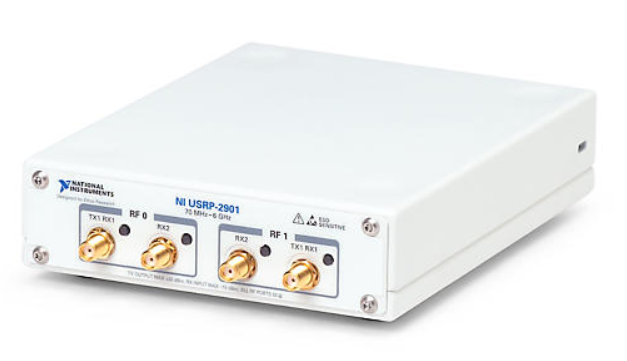
\includegraphics[width=0.4\textwidth]{Figuras/usrp.PNG}   
	\caption{NI USRP-2901 \citep{ettus}. }
	\label{fig:figura90}
\end{figure}